\documentclass[a4paper,11pt]{article}
\usepackage[utf8]{inputenc}
\usepackage[T1]{fontenc}
\usepackage[english]{babel}
\usepackage[margin=2.5cm]{geometry}
\usepackage{graphicx}
\usepackage{longtable}
\usepackage{float}
\usepackage{url}
\usepackage{parskip}
\usepackage{tikz}
\usetikzlibrary{arrows.meta,positioning}

\begin{document}

\begin{titlepage}
\noindent
\includegraphics[width=0.5\textwidth]{img/image1.png}

\vspace*{5cm}
\begin{center}
  {\Large\bfseries IMPLEMENTATION OF IFJ26 IMPERATIVE LANGUAGE TRANSLATOR\par}
  \vspace{0.5cm}
  Variant: TRP-izp\par
  \vspace{1.2cm}
  {\large\bfseries Formal languages and translators\par}
\end{center}

\vspace{3cm}
\noindent\begin{tabular*}{\textwidth}{@{\extracolsep{\fill}} l l l l}
  Name & BUT login & Personal number & Points \\
  \hline
  \textbf{Alexandr Jordán} & xjordaa00 & 282201 & 25 \\
  Matyáš Filip Jurásek & xjurasm00 & 282796 & 25 \\
  Patrik Lisál & xlisalp00 & 269966 & 25 \\
  Michal Jáger & xjagerm00 & 282462 & 25 \\
\end{tabular*}

\vspace{1cm}
\noindent Extensions: EXT\_FUNEXP, EXT\_BOOLTHEN

\noindent GitHub link: \url{https://github.com/alexandrjordan0/ifj26}
\end{titlepage}


\section{Team work}

The team was formally founded in the BUT information system by Matyáš Filip Jurásek
and the team leader is Alexandr Jordán. The leader is responsible for the development
plan, the division of work, the rules of cooperation, the repository infrastructure,
the deadlines and the merging of code.

At the beginning of the semester we made a development plan with milestones according
to the assignment, that is the registration of the variant on 30 September, the trial
submission on 19 November and the final submission on 27 November. We divided the
translator into modules and every module has its responsible member.

\subsection{Division of work}

Patrik Lisál implemented the lexical analyser in scanner.c. Michal Jáger
implemented the hashtable and the symbol table in hashtable.c and
symtable.c and the module of error codes error.c. Matyáš Filip Jurásek
implemented the syntactic and semantic analysis using recursive descent in
parser.c. Alexandr Jordán implemented the precedence analysis of expressions in
precedence.c, the code generator in codegenerator.c, the dynamic string
in str.c and the main program main.c, which connects all modules
together.

\subsection{Repository and workflow}

We use a repository on GitHub with a Makefile, the configuration of the Clang
formatter and continuous integration in GitHub Actions, which checks on every push and
pull request that the project can be compiled. Nobody commits directly into the branch
main. Every change is made on its own branch feat/ or fix/ and gets into main through a
pull request after it is approved by another member of the team. Commit messages follow
the Conventional Commits convention and the code is formatted by make format before it
is pushed.

Pull requests are reviewed by other members of the team and conflicts are resolved
when merging branches. We tested the translator on example programs with the reference
interpreter and before every submission we checked the archive with the script
is\_it\_ok.sh. Until the trial submission 22 pull requests were created.

\section{Module description}

\subsection{Scanner}

Scanner is implemented in two files, scanner.c and scanner.h. It reads
source code from standard input and converts it into tokens that are used by the parser.
The header file defines the token types, the Token structure and the public
functions of the scanner. Every token stores its type, its value and its position in the
source code. The position is line and column.

The main function get\_next\_token reads one token at a time. Token recognition
is implemented as a finite-state automaton, which is shown in figures \ref{fig:fsm1},
\ref{fig:fsm2} and \ref{fig:fsm3}. Each new token starts in state S\_START and
then moves to a state that handles the current construct. Separate states are used for
identifiers, numbers, strings, comments and operators. This keeps the recognition logic
separated and makes it easier to handle different lexical rules.

Keywords are recognized using a table of known words. If a read identifier is not present
in this table, it is returned as TOKEN\_IDENTIFIER. The scanner also recognizes
integer and double literals, including digit separators. Before converting a number to its
final C value, underscores are removed from the temporary buffer. Single-line strings
support the required escape sequences, while triple-quoted strings are read as multiline
string literals without interpreting escapes.

The scanner handles both line comments and nested block comments. A line comment is
ignored until the end of the line. Block comments are processed using a nesting counter,
so another block comment can appear inside an existing one. If a block comment contains a
newline, it is treated as a logical end of line according to the IFJ26 specification.

Indentation is handled separately at the beginning of each line. The scanner stores
indentation levels in a stack. When a new line is more indented, TOKEN\_INDENT is
generated. When indentation decreases, one or more TOKEN\_DEDENT tokens are
generated. Invalid indentation levels and tabs before code are reported as lexical errors.
Newlines inside parentheses are ignored for logical line separation, which allows
expressions and function calls to span multiple physical lines.

The parser uses get\_next\_token to consume tokens. Sometimes the parser needs to
inspect the next token, without consuming it, to decide which parsing rule to use. For
this purpose, peek\_next\_token stores one token in a lookahead variable and
returns a pointer to it. Repeated calls return the same buffered token, and the next call
of get\_next\_token consumes it. Dynamically allocated string values are released
by token\_free when the parser no longer needs the token. Function
scanner\_init resets the scanner position and its indentation and character
lookahead state before scanning starts.

\subsection{Hashtable and symtable}

The module includes two .c/.h pairs of files, hashtable and symtable.

Hashtable serves as an abstract data type that stores any key/value pairs and indexes them
using a hash function. We used the sdbm hash function, because it is simple, fast and has
good distribution \cite{sdbm}. The function hashtable\_init creates a new
hashtable and hashtable\_delete deletes whole table and frees all allocated
memory.

The function hashtable\_add inserts a new item to hashtable. When adding a new
item to hashtable, the load factor is checked. Because it is a variant with implicit
chaining of items, we do not wait until table is full. If load factor exceeds 70\,\%,
capacity of hashtable is doubled and all items are rehashed. In case of collisions, we use
linear probing -- value is stored at the next free position.

In our application single items are never deleted from hashtable so we do not consider
that. Because of that, no tombstones are needed. hashtable\_search returns value
with given key.

Symtable is ADT over hashtable and the rest of the translator uses symtable.h as
API. Hashtable and symtable could be merged together, but we chose to separate them
because now it is more clear.

Symtable consists of global hashtable for functions and stack of scopes for variables. The
stack of scopes is implemented as a linked list where every scope has its own hashtable of
variables and a link to its parent. Variables are always stored in current (innermost
open) scope. In VarInfo are information about a variable -- type, mutability
(var is mutable, val or function parameter not) and
scope\_depth. In FuncInfo is stored name, information about parameters,
return\_type of function and is\_defined flag, which is set to true if
the function has been fully implemented.

When function symtable\_find\_var searches for variables, it starts in the
deepest scope (allowing shadowing). Function symtable\_find\_var\_current\_scope
searches only in current scope (for redefinition detection, error 4). The function name,
parameter types and parameter names are copied, so the table owns them and the function
symtable\_free frees them using callback func\_free.

\subsection{Parser}

The module includes one pair of .c/.h files, parser.c and parser.h.
Module parser is used for syntactic and semantic analysis and uses modules symtable,
precedence, scanner and codegenerator. Parser uses recursive descent based on an LL
grammar for syntactic analysis. For rule CommandSimple parser uses auxiliary function
called parse\_command\_simple\_id where it calls peek\_next\_token
function from the scanner module, getting look ahead token and deciding on correct rule
usage. For parsing expressions (including function calls) parser uses separate precedence
parsing.

Parser works in two separate so-called runs. In first run parser takes and saves
declaration (heads) of all the functions in source file and adds this information into
symtable while ignoring bodies of said functions. In the second run parser analyses bodies
of the functions, their syntax, analyses command semantics, evaluates return commands and
compares its return type to its declared type. In case where the return type was not
declared, parser derives its return type from structure block\_result.

Non-terminals: Program, Prolog, FuncSet, Func, MainAnot, MainAnotEOL, ParamSet, ParamNext,
Param, FuncParams, ParamNextRest, Type, RetType, Body, Variable, Value, VariableType,
ValueType, Block, Expression, CommandSet, CommandNext, Command, CommandSimple,
CommandComplex, RetCommand, IfStatement, VolElse, ElseBlock, WhileStatement, Separator.

Terminals: INDENT, DEDENT, EOF, EOL, IMPORT, DOT, MUL, LPAR, RPAR, COMMA, COLON,
SEMICOLON, ID, DEF, VAR, VAL, MAIN, ASSIGN, INT, STRING, DOUBLE, UNIT, BOOLEAN, litUNIT,
IF, ELSE, THEN, WHILE, DO, RETURN.

The LL(1) grammar is shown in table \ref{tab:grammar} and the LL table in figures
\ref{fig:ll1} to \ref{fig:ll4}.

{\small
\begin{longtable}{r p{0.52\textwidth} p{0.36\textwidth}}
  \caption{LL(1) grammar}\label{tab:grammar}\\
  \hline
  N & Rule & Predict(Rule) \\
  \hline
  \endfirsthead
  \hline
  N & Rule & Predict(Rule) \\
  \hline
  \endhead
  \hline
  \endfoot
  1 & Program $\rightarrow$ Prolog FuncSet EOF & \{IMPORT\} \\
2 & Prolog $\rightarrow$ IMPORT ID DOT MUL EOL & \{IMPORT\} \\
3 & FuncSet $\rightarrow$ Func FuncSet & \{MAIN, DEF\} \\
4 & FuncSet $\rightarrow$ $\varepsilon$ & \{EOF\} \\
5 & Func $\rightarrow$ MainAnot DEF ID FuncParams RetType ASSIGN Body & \{MAIN, DEF\} \\
6 & FuncParams $\rightarrow$ litUNIT & \{litUNIT\} \\
7 & FuncParams $\rightarrow$ LPAR ParamSet RPAR & \{LPAR\} \\
8 & MainAnot $\rightarrow$ MAIN MainAnotEOL & \{MAIN\} \\
9 & MainAnot $\rightarrow$ $\varepsilon$ & \{DEF\} \\
10 & MainAnotEOL $\rightarrow$ EOL & \{EOL\} \\
11 & MainAnotEOL $\rightarrow$ $\varepsilon$ & \{DEF\} \\
12 & ParamSet $\rightarrow$ Param ParamNext & \{ID\} \\
13 & ParamSet $\rightarrow$ $\varepsilon$ & \{RPAR\} \\
14 & ParamNext $\rightarrow$ COMMA ParamNextRest & \{COMMA\} \\
15 & ParamNext $\rightarrow$ $\varepsilon$ & \{RPAR\} \\
16 & ParamNextRest $\rightarrow$ Param ParamNext & \{ID\} \\
17 & ParamNextRest $\rightarrow$ $\varepsilon$ & \{RPAR\} \\
18 & Param $\rightarrow$ ID COLON Type & \{ID\} \\
19 & Type $\rightarrow$ INT & \{INT\} \\
20 & Type $\rightarrow$ STRING & \{STRING\} \\
21 & Type $\rightarrow$ DOUBLE & \{DOUBLE\} \\
22 & Type $\rightarrow$ UNIT & \{UNIT\} \\
23 & Type $\rightarrow$ BOOLEAN & \{BOOLEAN\} \\
24 & RetType $\rightarrow$ COLON Type & \{COLON\} \\
25 & RetType $\rightarrow$ $\varepsilon$ & \{ASSIGN\} \\
26 & Body $\rightarrow$ Expression EOL & \{ID, MINUS, litINT, litDOUBLE, litSTRING, litUNIT, NOT, TRUE, FALSE, LPAR\} \\
27 & Body $\rightarrow$ EOL Block & \{EOL\} \\
28 & Variable $\rightarrow$ VAR ID VariableType ASSIGN Expression & \{VAR\} \\
29 & VariableType $\rightarrow$ COLON Type & \{COLON\} \\
30 & VariableType $\rightarrow$ $\varepsilon$ & \{ASSIGN\} \\
31 & Value $\rightarrow$ VAL ID ValueType ASSIGN Expression & \{VAL\} \\
32 & ValueType $\rightarrow$ COLON Type & \{COLON\} \\
33 & ValueType $\rightarrow$ $\varepsilon$ & \{ASSIGN\} \\
34 & Block $\rightarrow$ INDENT Command DEDENT & \{INDENT\} \\
35 & CommandSet $\rightarrow$ Command & \{VAR, VAL, RETURN, ID, MINUS, litINT, litDOUBLE, litSTRING, litUNIT, NOT, TRUE, FALSE, LPAR, IF, WHILE, EOL\} \\
36 & CommandSet $\rightarrow$ $\varepsilon$ & \{DEDENT\} \\
37 & CommandNext $\rightarrow$ Separator CommandSet & \{EOL, SEMICOLON\} \\
38 & CommandNext $\rightarrow$ $\varepsilon$ & \{DEDENT\} \\
39 & Command $\rightarrow$ CommandSimple CommandNext & \{VAR, VAL, RETURN, ID, MINUS, litINT, litDOUBLE, litSTRING, litUNIT, NOT, TRUE, FALSE, LPAR\} \\
40 & Command $\rightarrow$ CommandComplex CommandSet & \{IF, WHILE\} \\
41 & Command $\rightarrow$ EOL CommandSet & \{EOL\} \\
42 & CommandSimple $\rightarrow$ Variable & \{VAR\} \\
43 & CommandSimple $\rightarrow$ Value & \{VAL\} \\
44 & CommandSimple $\rightarrow$ RETURN RetCommand & \{RETURN\} \\
45 & CommandSimple $\rightarrow$ ID ASSIGN Expression & \{ID\} \\
46 & CommandSimple $\rightarrow$ Expression & \{ID, MINUS, litINT, litDOUBLE, litSTRING, litUNIT, NOT, TRUE, FALSE, LPAR\} \\
47 & CommandComplex $\rightarrow$ IfStatement & \{IF\} \\
48 & CommandComplex $\rightarrow$ WhileStatement & \{WHILE\} \\
49 & RetCommand $\rightarrow$ Expression & \{ID, MINUS, litINT, litDOUBLE, litSTRING, litUNIT, NOT, TRUE, FALSE, LPAR\} \\
50 & RetCommand $\rightarrow$ $\varepsilon$ & \{EOL, SEMICOLON, DEDENT\} \\
51 & Separator $\rightarrow$ SEMICOLON & \{SEMICOLON\} \\
52 & Separator $\rightarrow$ EOL & \{EOL\} \\
53 & IfStatement $\rightarrow$ IF Expression THEN EOL Block VolElse & \{IF\} \\
54 & VolElse $\rightarrow$ ELSE ElseBlock & \{ELSE\} \\
55 & VolElse $\rightarrow$ $\varepsilon$ & \{VAR, VAL, RETURN, ID, MINUS, litINT, litDOUBLE, litSTRING, litUNIT, NOT, TRUE, FALSE, LPAR, IF, WHILE, DEDENT, EOL\} \\
56 & ElseBlock $\rightarrow$ EOL Block & \{EOL\} \\
57 & ElseBlock $\rightarrow$ IfStatement & \{IF\} \\
58 & WhileStatement $\rightarrow$ WHILE Expression DO EOL Block & \{WHILE\} \\

\end{longtable}
}

\begin{figure}[H]
  \centering
  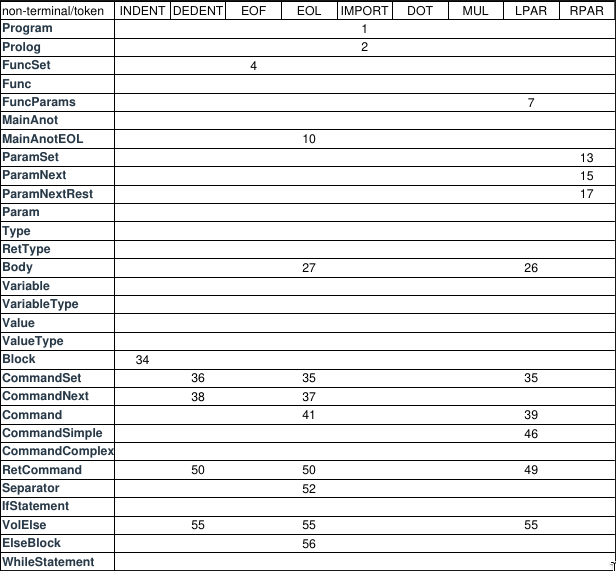
\includegraphics[width=0.8\textwidth]{img/image5.png}
  \caption{LL table, part 1}\label{fig:ll1}
\end{figure}
\begin{figure}[H]
  \centering
  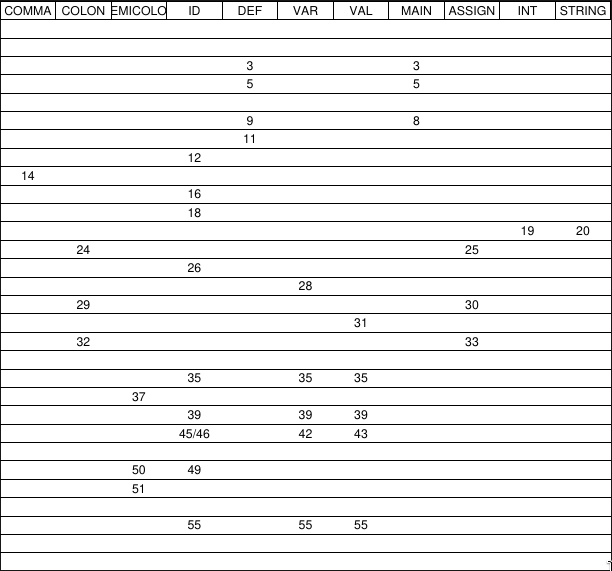
\includegraphics[width=0.8\textwidth]{img/image6.png}
  \caption{LL table, part 2}\label{fig:ll2}
\end{figure}
\begin{figure}[H]
  \centering
  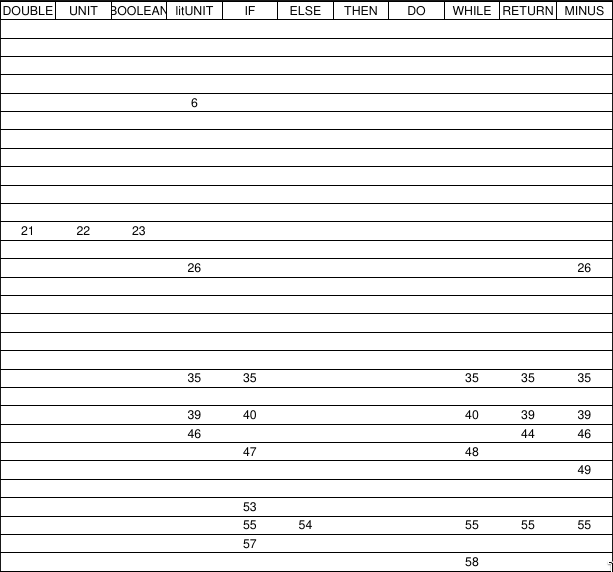
\includegraphics[width=0.8\textwidth]{img/image7.png}
  \caption{LL table, part 3}\label{fig:ll3}
\end{figure}
\begin{figure}[H]
  \centering
  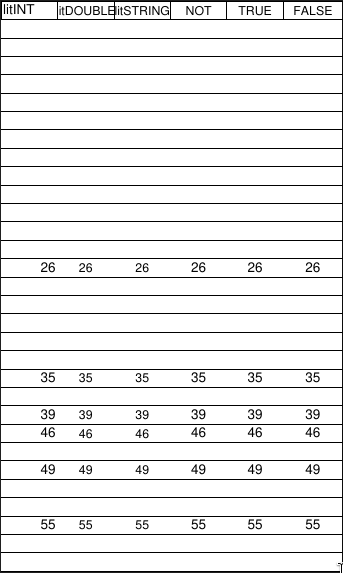
\includegraphics[width=0.45\textwidth]{img/image8.png}
  \caption{LL table, part 4}\label{fig:ll4}
\end{figure}

\subsection{Precedence analysis of expressions}

Expressions are processed by bottom up operator precedence analysis in the module
precedence.c. The parser passes control to it by calling the function
parse\_expression, which gets the first token of the expression and the symbol
table, processes the whole expression and returns its data type together with the first
token after the expression, on which the parser continues. In case of an error it returns
code 2 for a syntax error, 3 to 7 for semantic errors and 99 for an internal error.

The analysis works with a stack implemented as a linked list. The stack holds terminals,
the nonterminal E, the mark < which marks the beginning of a handle and
the bottom \$. Every item also stores its data type. The action shift, equal,
reduce or error is chosen by the precedence table of size $18 \times 18$ according to the
topmost terminal on the stack and the current input symbol. The end of an expression is
not searched separately. Every token that does not belong to the expression, for example
end of line, then, do or comma, behaves as \$.

Unary minus is distinguished from binary minus by the previous symbol. If it is not
preceded by an operand or a right parenthesis, it is a unary operator. An identifier
followed by a left parenthesis is a function call. Its arguments are processed by a
recursive call of parse\_expression and their count and types are checked against
the signature in the symbol table. A mismatch results in error 5.

Priorities and associativity of operators, which follow from the precedence table, are
shown in table \ref{tab:priority}. The full precedence table is shown in figure
\ref{tab:prec}. Symbol $<$ means shift, $=$ means equal for matching parentheses and $>$
means reduce.

\begin{table}[H]
  \centering
  \begin{tabular}{c l l}
    \hline
    Level & Operators & Associativity \\
    \hline
    1 & !, unary - & right \\
    2 & *, / & left \\
    3 & +, - & left \\
    4 & <, >, <=, >= & none \\
    5 & ==, != & none \\
    6 & \&\& & left \\
    7 & || & left \\
    \hline
  \end{tabular}
  \caption{Priority of operators from the highest}
  \label{tab:priority}
\end{table}

\begin{figure}[H]
  \centering
  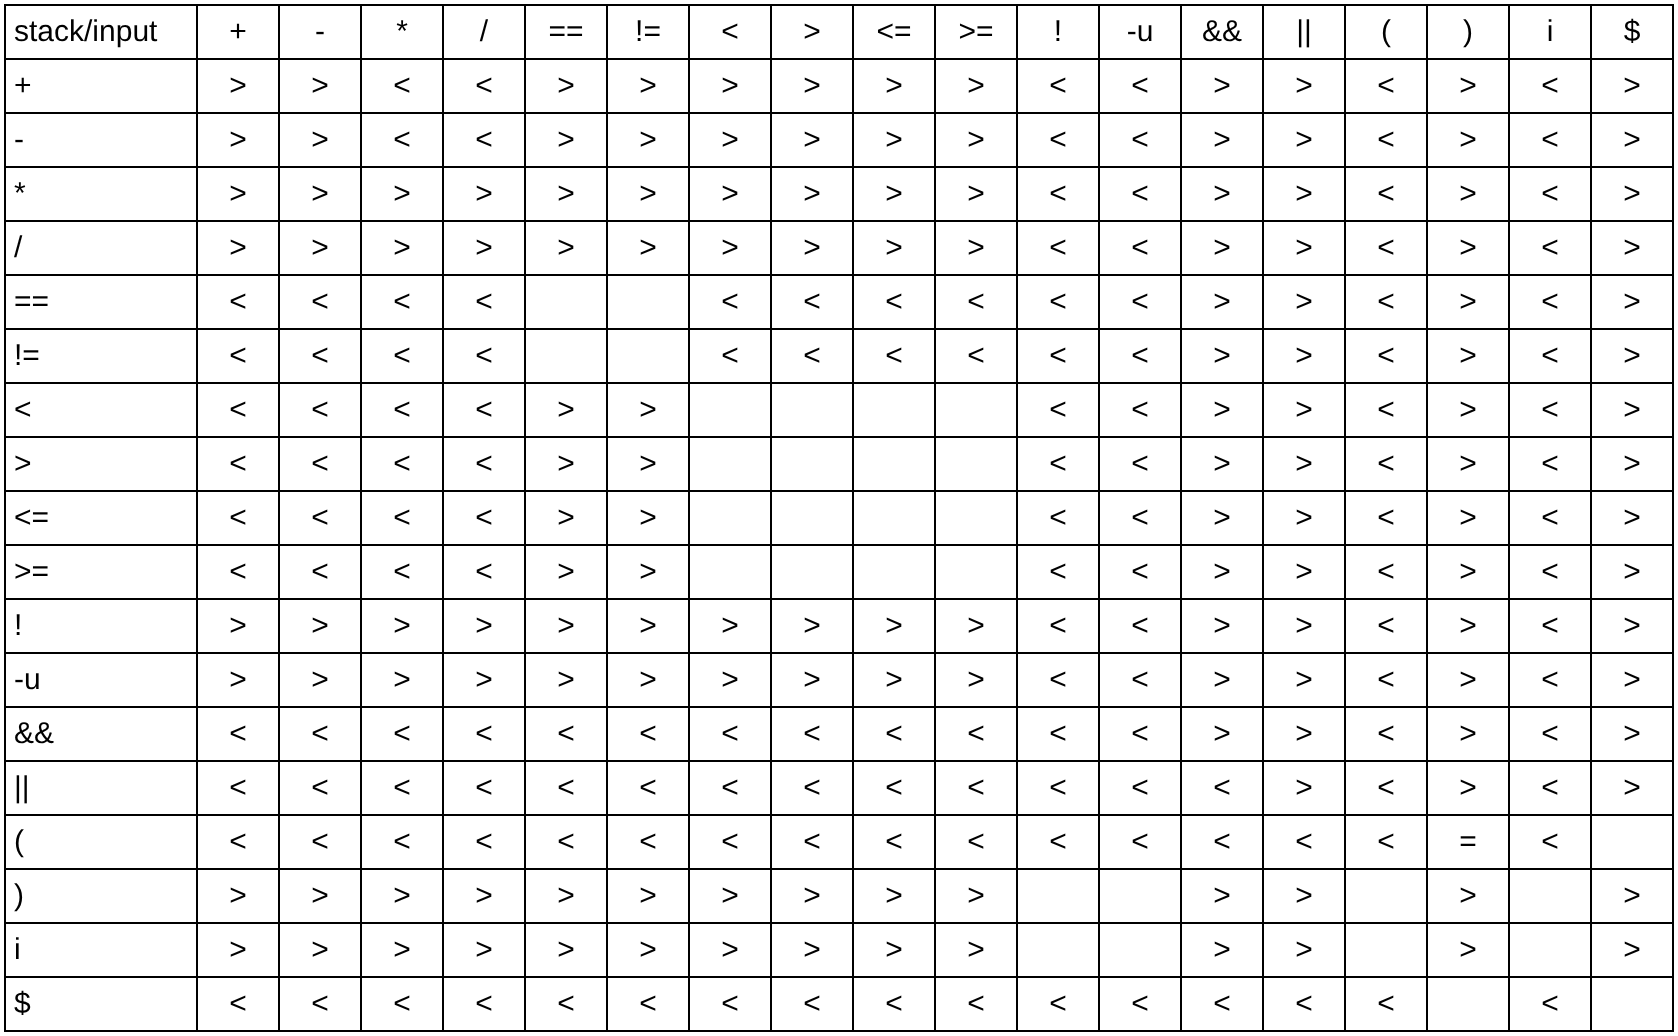
\includegraphics[width=\textwidth]{img/prec.png}
  \caption{Precedence table, the row is the topmost terminal on the stack, the column is the input symbol, an empty cell means an error}
  \label{tab:prec}
\end{figure}

Type checking is done during every reduction. Arithmetic operators accept types
Int and Double and operator + also accepts two strings, which
are concatenated. A combination of Int and Double leads to the only
allowed implicit conversion from Int to Double. Relational operators
return Boolean, operators == and != compare operands of the
same type or Int with Double and logical operators accept only
Boolean. Any other combination is error 6. Chaining of non associative
operators, for example a < b < c, is a syntax error.

The precedence analysis also drives the code generation of an expression. Shift of an
operand generates a push of the value onto the data stack and reduction of an operator
generates the corresponding stack instruction. Operators \&\& and ||
are evaluated with short circuit. The left operand is tested already when the operator is
shifted and the labels which wait for reduction are kept in a separate stack of the
module.

\subsection{Code generator}

The generator in the module codegenerator.c creates stack based IFJcode26 code
directly during the syntactic analysis, without an intermediate tree. The parser and the
precedence analysis call functions of the generator at the moment when they recognize the
corresponding construct. Cooperation of the modules is shown in figure \ref{fig:arch}.

\begin{figure}[H]
  \centering
  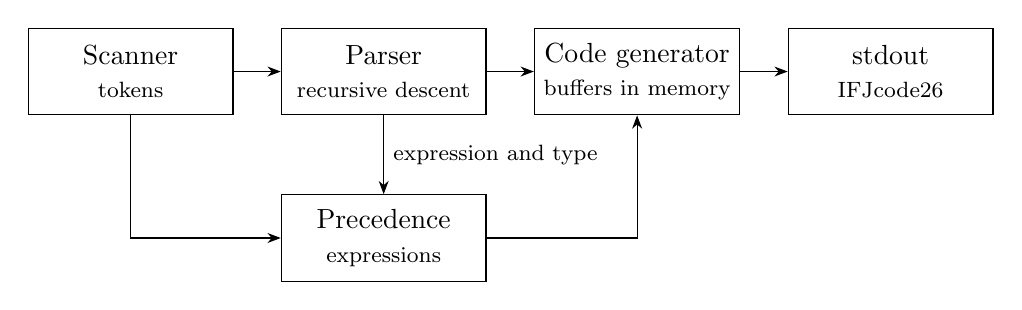
\begin{tikzpicture}[
      node distance=10mm and 6mm,
      box/.style={draw, minimum width=26mm, minimum height=11mm, align=center},
      arr/.style={-{Stealth}}
    ]
    \node[box] (scanner) {Scanner\\\footnotesize tokens};
    \node[box, right=of scanner] (parser) {Parser\\\footnotesize recursive descent};
    \node[box, right=of parser] (gen) {Code generator\\\footnotesize buffers in memory};
    \node[box, right=of gen] (out) {stdout\\\footnotesize IFJcode26};
    \node[box, below=of parser] (prec) {Precedence\\\footnotesize expressions};
    \draw[arr] (scanner) -- (parser);
    \draw[arr] (parser) -- (gen);
    \draw[arr] (gen) -- (out);
    \draw[arr] (parser) -- node[right, font=\footnotesize] {expression and type} (prec);
    \draw[arr] (prec) -| (gen);
    \draw[arr] (scanner) |- (prec);
  \end{tikzpicture}
  \caption{Cooperation of translator modules}
  \label{fig:arch}
\end{figure}

The generated program starts with the header .IFJcode26 and the definition of
auxiliary global variables GF@\$tmp1, GF@\$tmp2 and
GF@\$last. It continues with the call of the function annotated with
@main and the end of the program, then user functions in the order of the source
code and finally built in functions. The whole code is assembled in buffers in memory and
it is written to the standard output only after a successful analysis, so no incomplete
output is produced in case of an error.

Local variables and function parameters are stored in the local frame under a name
composed of the identifier and the depth of the block, for example LF@x\$1.
Thanks to that, variables with the same name in nested blocks do not collide. The
instruction DEFVAR must not be executed twice, which would happen inside a loop,
so the generator collects declarations of the whole function in a separate buffer and
inserts them once at the beginning of its body without duplicates.

Every function starts with a label, creation and push of a new frame, declaration of
parameters and popping them from the data stack in reverse order. Arguments and the return
value are passed through the data stack. If return is not executed, the function
returns the value of the last expression statement, which the generator continuously
stores in GF@\$last. If the block ends with a definition, an assignment, a
condition or a loop, it returns nil, which is the unit value of type
Unit. A function with return type Unit drops the computed value and
returns the unit value, also in the case of a return statement.

Conditions and loops use labels with a number from a global counter, for example
\$else\$N, \$endif\$N, \$while\$N and
\$endwhile\$N, so they are unique at any level of nesting. The condition is
evaluated onto the stack and when its value is false, the program jumps to the
else branch or behind the end of the loop.

Expressions are translated to stack instructions. Concatenation of strings has no stack
variant, so the operands go through auxiliary global variables and the instruction
CONCAT. The implicit conversion from Int to Double works for the
operand on the top of the stack and also for the one below it. Type Int is 32 bit
as in Scala, so the result of integer arithmetic is adjusted by the auxiliary function
\$wrap32.

Built in functions are generated as subroutines with a label starting with the character
\$, so they do not collide with user functions. Function subStr checks
its bounds and when they are violated, it ends the program with runtime error 40.
Functions readInt and readDouble return zero on invalid input.

\subsection{Known limitations}

A call of a function without a declared return type before its definition is not
supported. At that moment the return type of the function is not derived yet, so the
translator reports error 6, although the program is valid.

\section{AI policy}

We used LLMs (Anthropic Claude, Google Gemini, OpenAI ChatGPT) for assignment explanation
and for generating unit tests.

We used AI mainly as a tool for solving bugs and for speeding up the development. When
a test failed or the translator returned a wrong error code, we gave the AI the
relevant part of the code together with the error and asked it to find the cause. It
also helped us with repetitive work, for example with writing test programs.
Every suggestion was reviewed by the author of the module before it was used and it went
through the same pull request review as any other change.

The biggest problem was that the AI often hallucinated. It suggested functions which do
not exist in our code, instructions which do not exist in IFJcode26 or rules of the
IFJ26 language which are not in the specification. It also could not understand the
context of the whole problem. It worked only with the part of the code that we gave it,
so its fixes often solved one case and broke another module, for example a change in
the parser which did not respect how the code generator works. In these situations we
did not use the suggestion or we changed it significantly and the final solution was
designed by us. The grammar, the LL table, the precedence table, the finite automaton
and the hashtable were made without AI.

\begin{thebibliography}{9}
  \bibitem{sdbm} Hash Functions [online]. York University, n.d. [viewed 25 October 2026].
  Available from: \url{http://www.cse.yorku.ca/~oz/hash.html}
\end{thebibliography}

\appendix
\section{Finite state automaton of the scanner}

\begin{figure}[H]
  \centering
  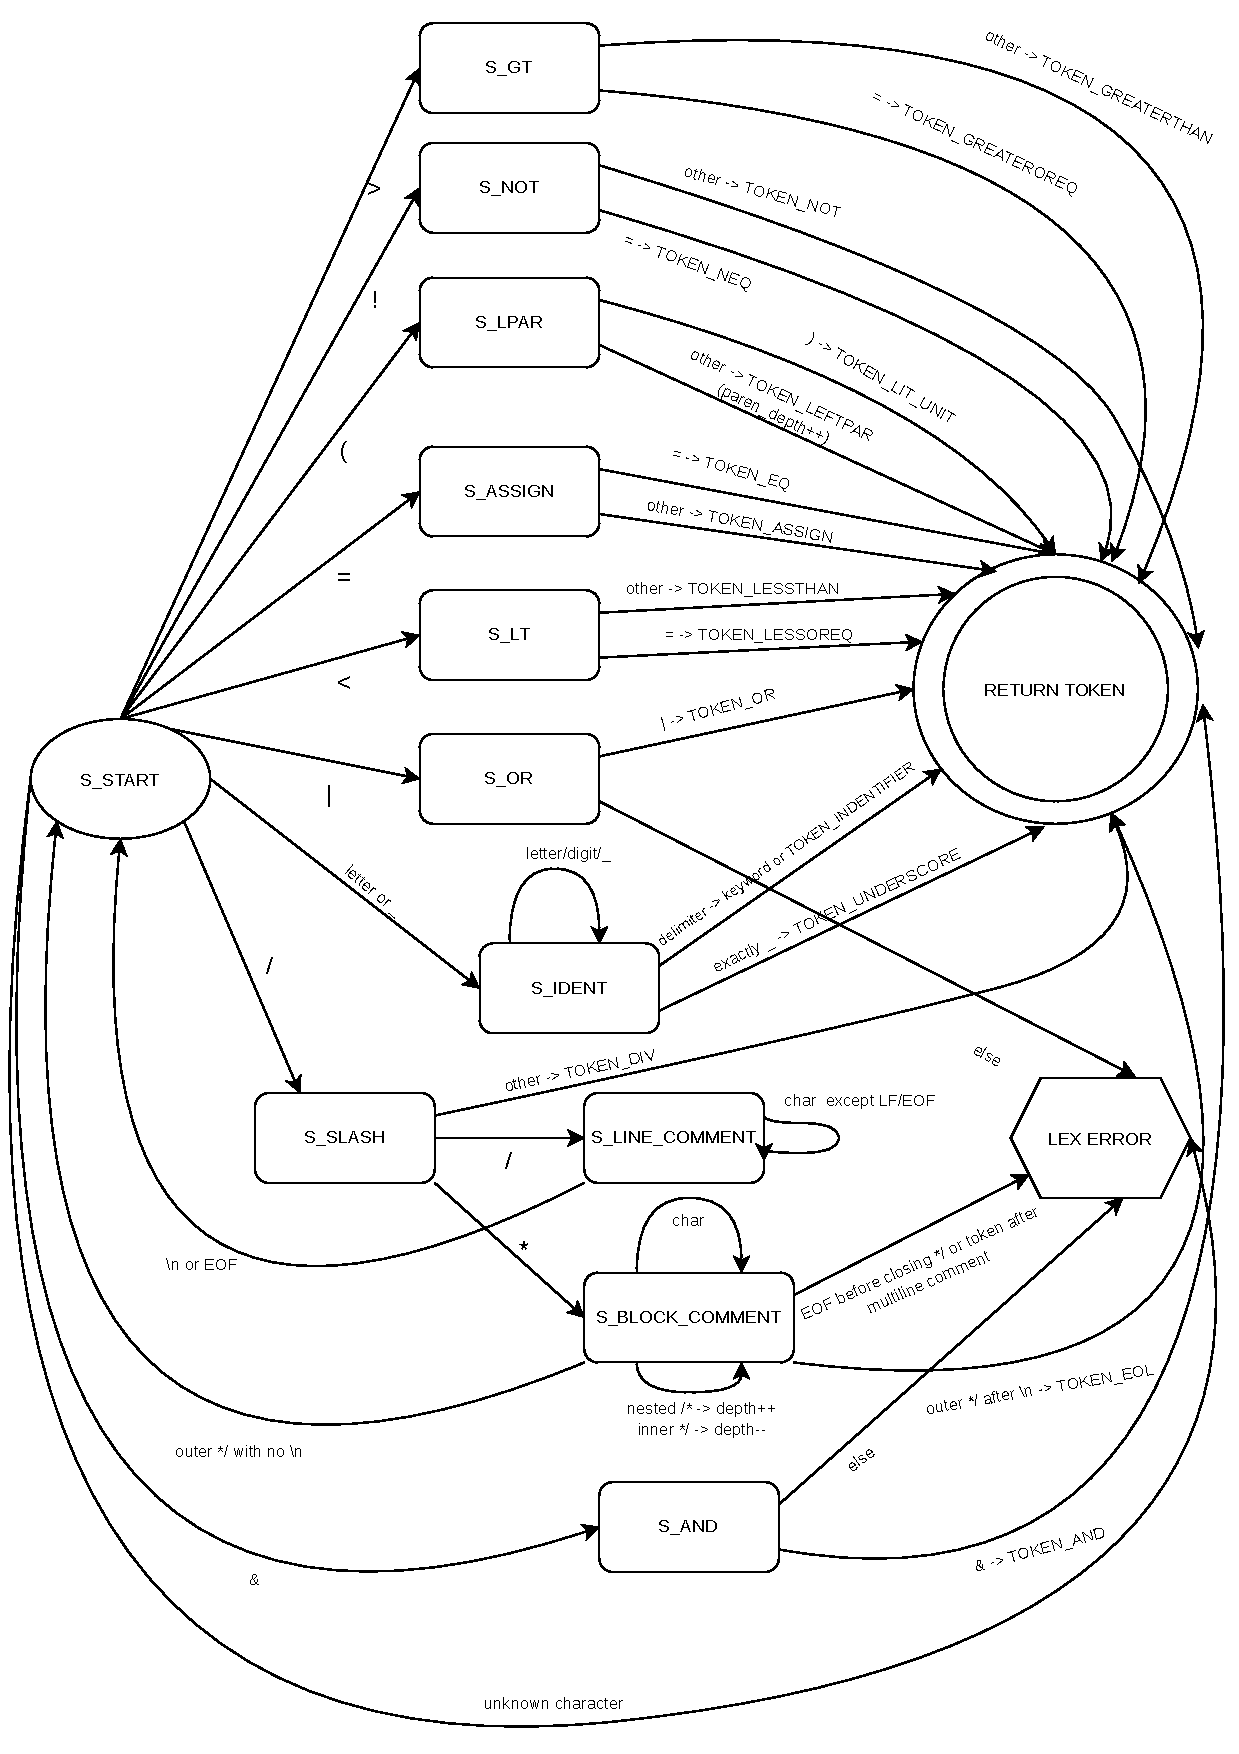
\includegraphics[page=1,width=\textwidth,height=0.8\textheight,keepaspectratio]{FSM_ifj.drawio.pdf}
  \caption{Finite state automaton, part 1}\label{fig:fsm1}
\end{figure}
\begin{figure}[H]
  \centering
  \includegraphics[page=2,width=\textwidth,height=0.8\textheight,keepaspectratio]{FSM_ifj.drawio.pdf}
  \caption{Finite state automaton, part 2}\label{fig:fsm2}
\end{figure}
\begin{figure}[H]
  \centering
  \includegraphics[page=3,width=\textwidth,height=0.8\textheight,keepaspectratio]{FSM_ifj.drawio.pdf}
  \caption{Finite state automaton, part 3}\label{fig:fsm3}
\end{figure}

\end{document}
